%%%%%%%%%%%%%%%%%%%%%%%%%%%%%%%%%%%%%%%%%%%%%%%%%%%%%%%%%%%%%%%%%%%%
\section{Data Acquisition System (DAQ) Overview (Georgia Karagiorgi \& David Newbold)}
\label{sec:fdsp-daq-ov}

\metainfo{2 Pages - largely generic but some highlighting of SP-specifics.}

%%%%%%%%%%%%%%%%%%%%%%%%%%%%%%%%%
\subsection{Introduction}
\label{sec:fdsp-daq-intro}

The overall DUNE Far Detector Data Acquisition System (DAQ) is
illustrated in Fig.~\ref{fig:daq-overview}.
\fixme{Describe figure here.}

Figure.~\ref{fig:daq-overview} illustrates the data flow and the
exchange of trigger and monitoring messages.



\begin{dunefigure}[DAQ Overview]{fig:daq-overview}
  {A generalized overview of high-level far detector \dword{daq}
    components showcasing the \dword{sp} \dword{detmodule}. 
    The electronics digitizes the detector signals and sends the data
    to the DAQ \dword{fe} readout hardware which sends the data to the
    \dword{fe} computing data receiver.
    The \dword{fe} readout hardware also processes the data stream to
    produce \dwords{trigprimitive} which are sent along with the data
    itself.
    The receiver sends the data to the \dword{ringbuffer} which is of
    sufficient size to retain the data long enough for a
    \dword{trigcommand} formed from the data itself to return.
    The receiver is also responsible to send out
    \dwords{trigcandidate}, formed from the \dwords{trigprimitive}, to
    the \dword{mtl} as input to forming a \dword{trigcommand}. 
    The \dword{mtl} forwards notification of this trigger process and
    accepts external \dwords{trigcandidate} from the \dword{gtl}.
    \Dwords{trigcommand} are then sent to the \dlong{eb} which queries
    the appropriate \dword{fe} computing units, aggregates the
    returned data and writes it to the \dword{diskbuffer} which is the
    interface to the Offline.}
% This PDF is made from the .dot of the same name.
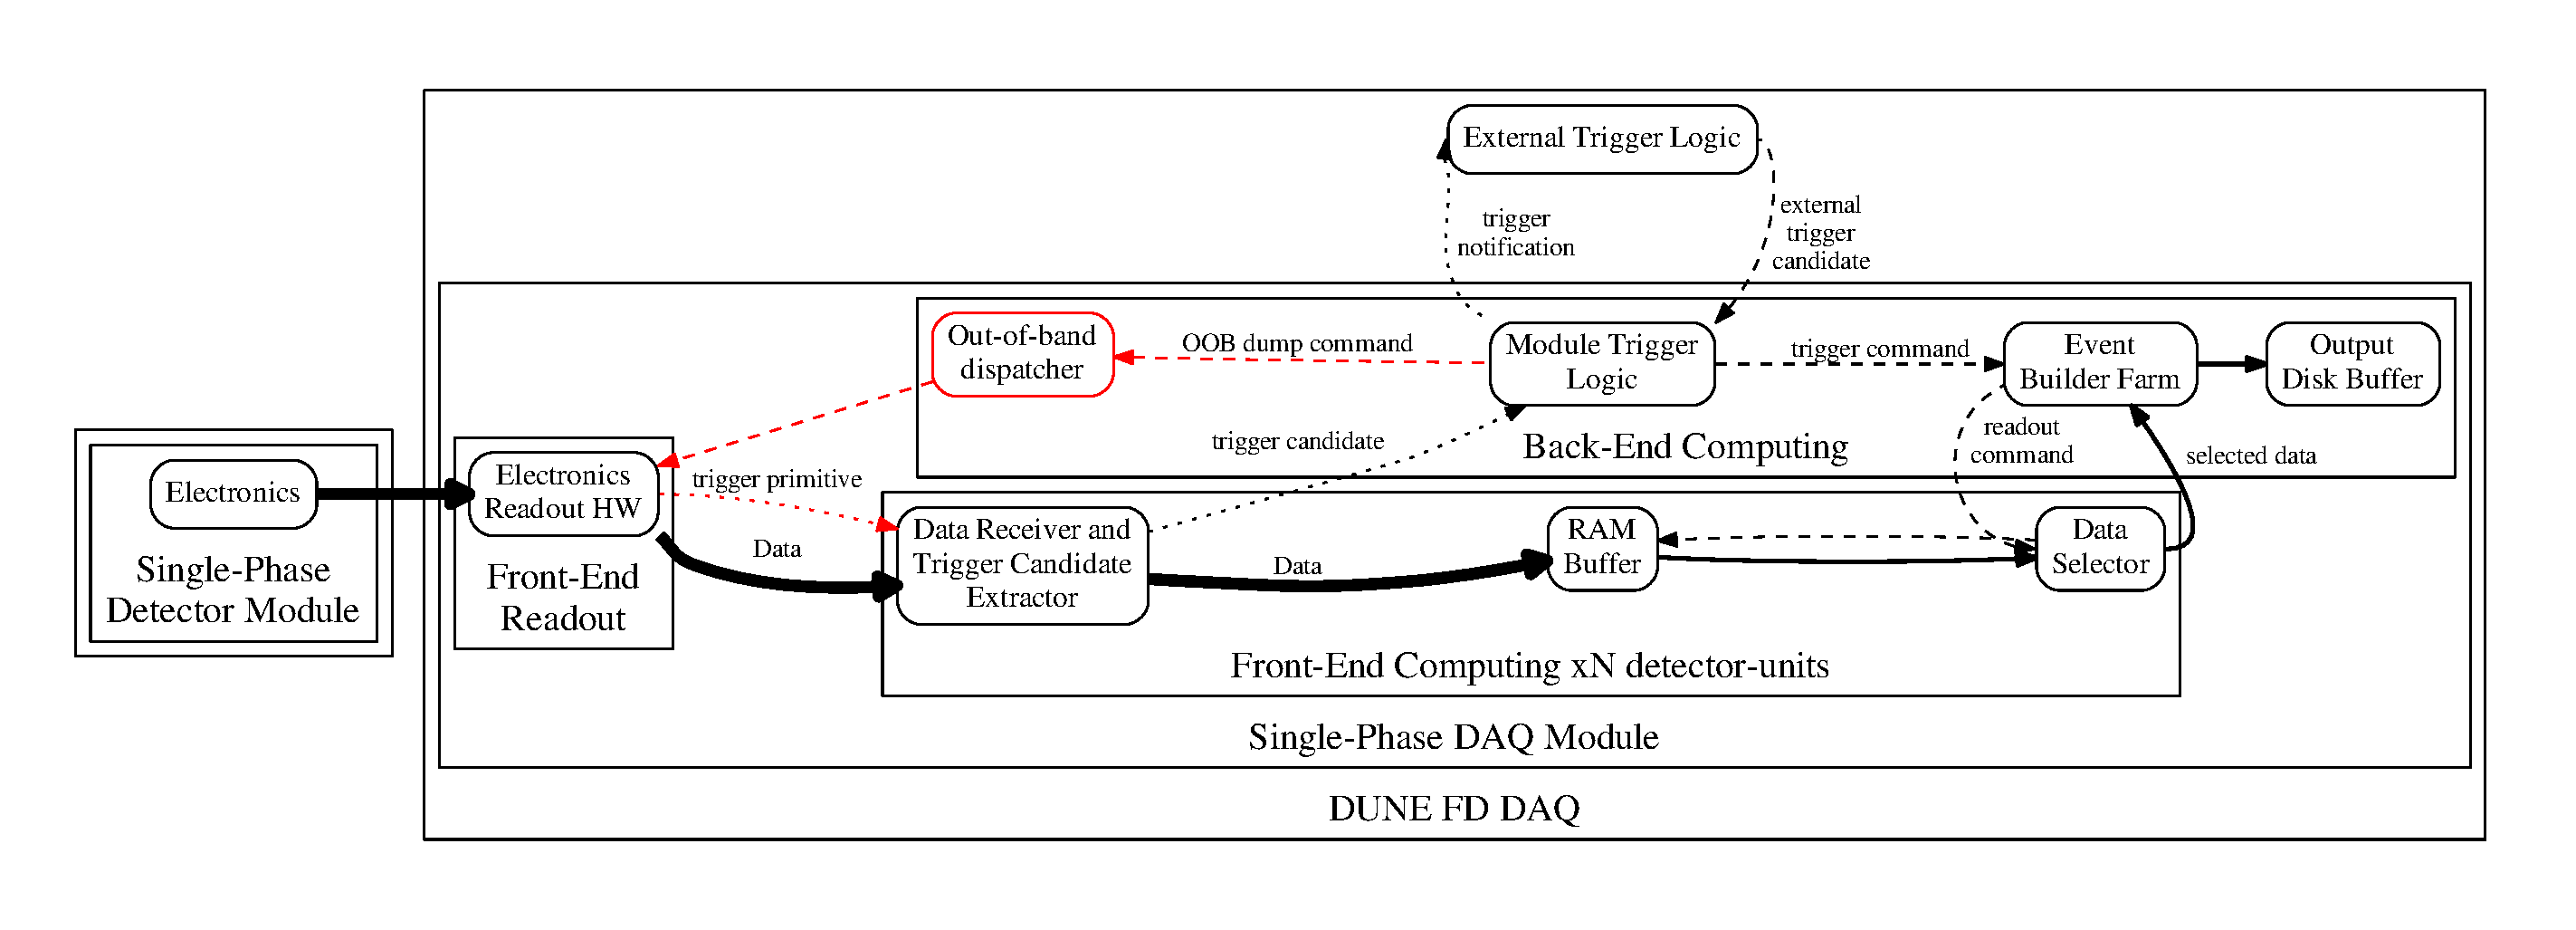
\includegraphics[width=0.8\textwidth]{daq-overview-sp.pdf}%
\end{dunefigure}


%%%%%%%%%%%%%%%%%%%%%%%%%%%%%%%%%%%%%

\subsection{Design Considerations}
\label{sec:fdsp-daq-des-consid}


\metainfo{Include: Raw data rate from WIBs, Josh's table of data volumes for each event type and the 30 PB/year offline limit. Space and thermal power limits.  Note, this table may be better put into Section~\ref{sec:fdsp-daq-design} to make this section more generic.}


The Data Acquisition System design must enable... 
...

\fixme{Anne suggests: Within this section add ref to requirements document when it's ready, and maybe list the most important half dozen in a table here). E.g.,}  

\begin{dunetable}
[Important requirements on the DAQ system design]
{p{0.8\textwidth}}
{pdphysicsparams}
{Important requirements on the DAQ system design}   
Requirement  \\ \toprowrule
  \\ \colhline
   \\ \colhline
 ...\\ 
\end{dunetable}

\fixme{By the end of the volume, for every requirement listed in this section, there should exist an explanation of how it will be satisfied.}


%%%%%%%%%%%%%%%%%%%%%%%%%%%%%%%%
\subsection{Scope}
\label{sec:fdsp-daq-scope}

\metainfo{This section may also wish to refer to Fig.~\ref{fig:daq-overview}.}

The scope of the Data Acquisition System includes the continued procurement of materials for, and the fabrication, testing, delivery and installation of the following systems: 

\fixme{Whatever the items are...}

\begin{itemize}
\item Readout electronics 
\item 
\end{itemize}


\newpage 
